\chapter{Flash Analysis}
\label{chp:Flash_Analysis}

%checklist:
% - introduction (goal)
% - Test setup
% - Proceedings in this chapter

The goal of this chapter is to find a method, capable of obtaining consistent measures of the environment from measured flashes. Secondary goals are to achieve this with the shortest flash and while using a small amount of computation power.

In this chapter, the platform is set-up as seen in figure \ref{fig:Flashcapturing}. 
D in the Figure represents the distance between the device and the reflecting surface (the wall in this case). All measurements presented in this chapter have been made in a darkroom, a room where no lights from outside can enter, so the test result won't get influenced by other illumination sources.
 
The set-up will first be used to get a reasonable understanding of what flashes look like and how settings of the flash generator influence the received flash. Then, several methods for obtaining a measure of the environment from flashes will be presented and compared. This chapter will conclude with the final settings used in the flash generator and an algorithm to obtain a consistent measure of the environment from the received flash.
\begin{figure}
	\centering     %%% not \center
	\subfigure[Test setup in illuminated environment]{\label{fig:Flashcapture_light}\includegraphics[width=60mm]{pics/Flashcapture_light.png}}
	\subfigure[Test set-up in dark environment]{\label{fig:Flashcapture_dark}\includegraphics[width=60mm]{pics/Flashcapture_dark.png}}
	\caption{Test set-up used to capture flashes in the darkroom.\label{fig:Flashcapturing}}
\end{figure}

\section{Flash properties}
\label{sec:Flash_generator}
The test set-up has several parameters which can affect the perceived flash: $T_{on}$ (on time of the LED), $I$ (brightness of the LED), $S_{PD}$ (sensitivity of the photodiode) and $D$ (distance between device and reflecting surface). This section shows how each of these parameters influences the received signal. Note that the period, $T$, is not present in the list as should not influence an individual flash as long as the flashes are not too close together.

Figure \ref{fig:InfOfTon} shows several responses for different $T_{on}$. The Figure shows that all signals closely match each other, until the light is turned off. This is a useful property as this means it's possible to reduce the $T_{on}$ with no influence on the signal, if the ending of the flash is not used.

Figure \ref{fig:InfOfI} shows the influence of using the different amplification circuits of the flash generator. It can be seen that the LED powered with more current (because of the smaller resistor) is perceived as brighter to the system than the lights powered with a smaller current. It's also observed that the LED powered with higher currents show up earlier to the system. This is because LEDs driven with higher currents turn on faster \cite{LED_on}. This means that if a lower LED current is used, a longer $T_{on}$ is required to obtain useful information.

Figure \ref{fig:InfOfD} shows a set of measured flashes at a variety of distances from the wall. It clearly shows that if the distance increases, the observed light decreases. This is logical, as when light travels longer distances, the relative intensity of the light decreases. 

Figure \ref{fig:InfOfPD} shows what happens when the different photodiodes are used. As expected, the RSS rises once we increase the gain on the photodiode. $S_{PD_3}$ almost instantly saturates as the gain is too strong when used in combination with $I_1$. $S_{PD_3}$ is therefore also displayed with in combination with $I_3$. Another noticeable change is the frequency of the ripple, caused by the amplifier. This change is expected, as the resistor in the feedback loop of the amplifier was changed.

\begin{figure}
	\centering     %%% not \center
	\subfigure[]{\label{fig:InfOfTon}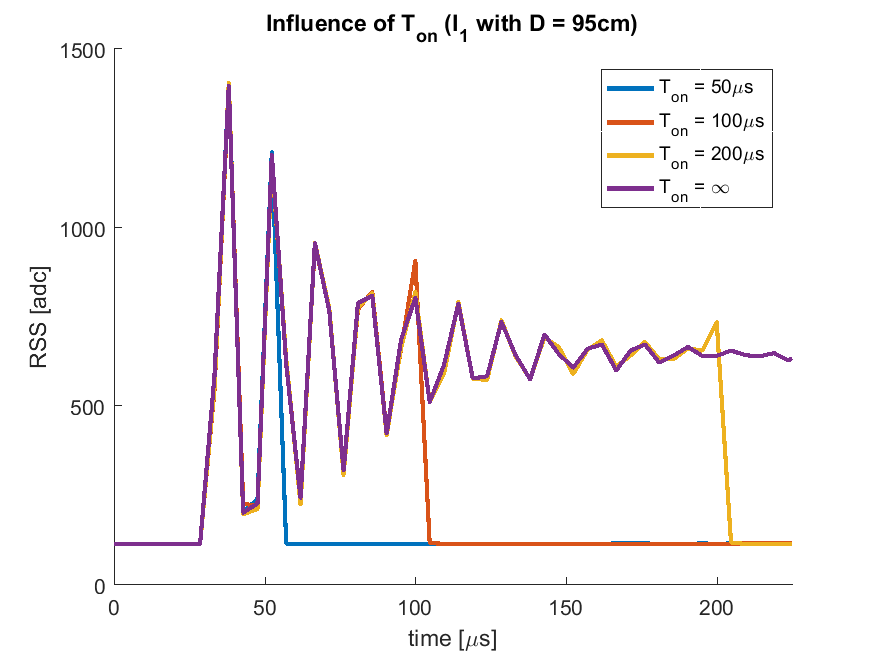
\includegraphics[width=60mm]{pics/InfluenceOfTon.png}}
	\subfigure[]{\label{fig:InfOfI}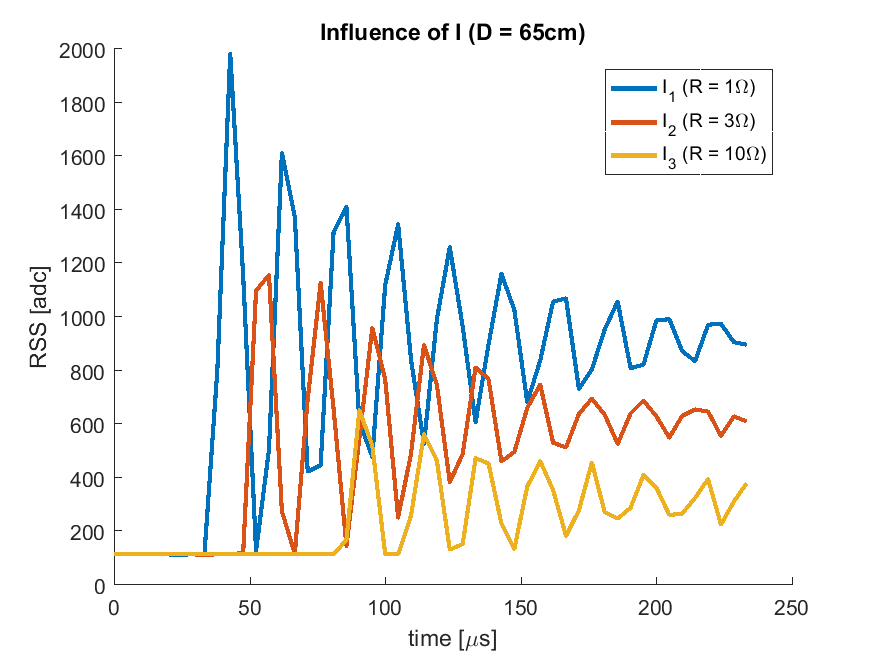
\includegraphics[width=60mm]{pics/InfluenceOfI.png}}
	\\
	\subfigure[]{\label{fig:InfOfD}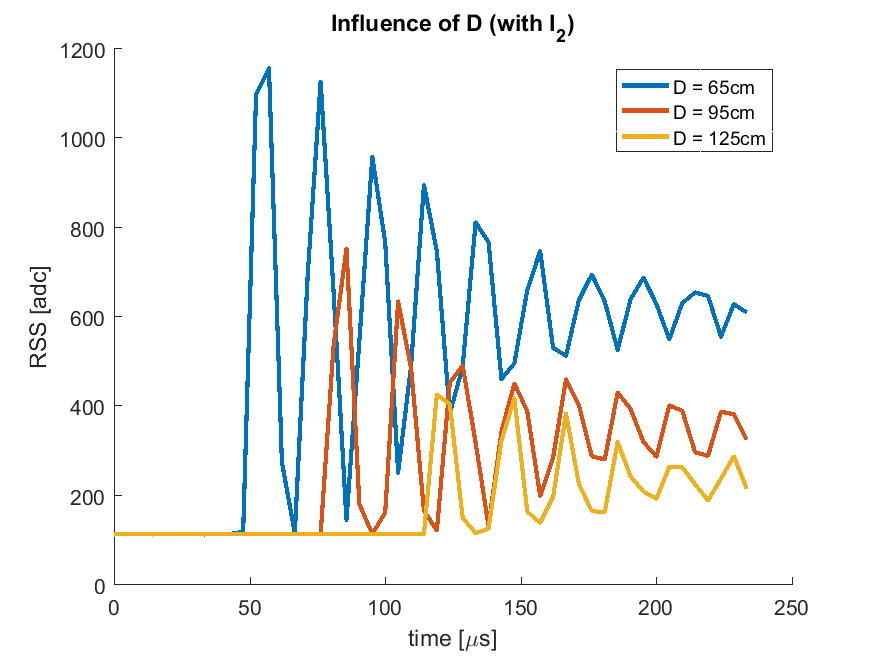
\includegraphics[width=60mm]{pics/InfluenceOfD.png}}
	\subfigure[]{\label{fig:InfOfPD}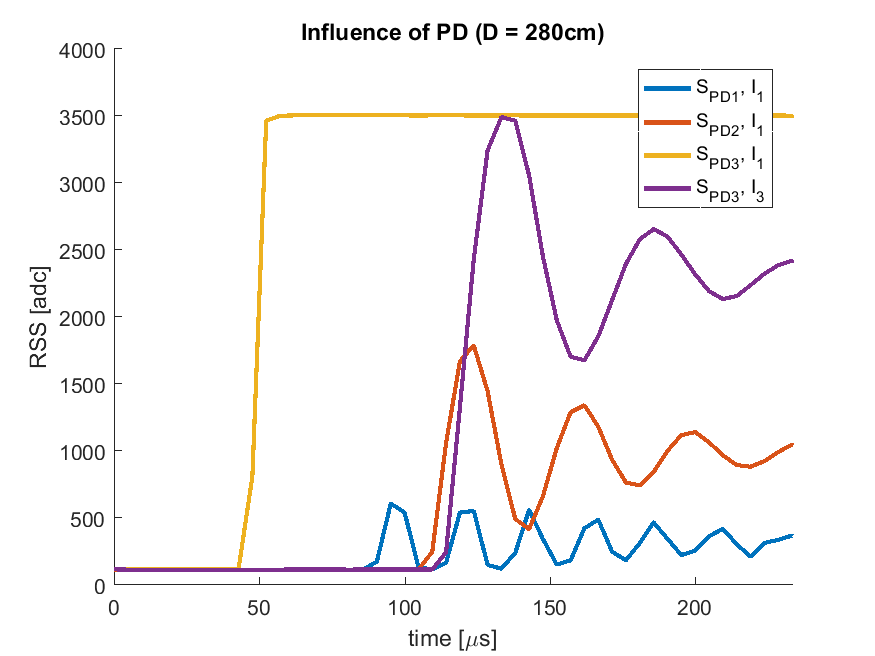
\includegraphics[width=60mm]{pics/InfluenceOfPD.png}}
	\caption{Several perceived flashes generated with different settings of $T_{on}$, $I_{LED}$, $D$ and $S_{PD}$.\label{fig:InfOf}}
\end{figure}

% properites checklist:
% - What happens if distance increases
%   + fig with multiple distances
% - What happens if t-on time increases
%   + fig with increasing t-on
% - What happens if intensity increases
%   + fig multiple 3 intensities
% sumarize in table 
% conclude:
% - 

\section{Flash features}
This section explores what kind of features can be extracted from a flash signal. It will then compare the methods based on required $T_{on}$, precision, detectability and computational complexity.

\subsection{Feature considerations}
The maximum of a flash response could contain useful information. Even though the light at the first maximum has not fully turned on yet, it still is some measure of the perceived light. This can be especially useful if the maximum of the flash always occurs at the exact same moment in time relative to the light turning on. If that's the case, then the maximum value of the first peak could provide us with enough information of the environment. If the maximum value of the first peak holds enough information, then a very small $T_{on}$ can be used to obtain this value, as decreasing $T_{on}$ does not significantly influence the height and form of the first peak.

Another possibility is to remove the oscillation of the signal with a low pass filter and then take the maximum value of the filtered signal. This method is less reliant on precise timing of the pulse. It also uses more samples of the signal and should therefore be able to obtain a value which better represents the reflections of the current environment than the maximum method. A downside to this method is that a filter designed to deal with one frequency of ripple, is not immediately suited to deal with the ripple frequencies of the other amplifiers

Another method considered is to use the area underneath the flash. This method has the advantage of being both simple and flexible. It does not matter if $T_{on}$ is chosen big or small, it will always give a reliable result if $T_{on}$ is not changed. It also does not care about the ripple frequency of the amplifier. This method simply sums all information available to obtain a measure of the reflections.

The final possibility considered is the filtered sum method. It first uses a filter to smooth the signal to then calculate the surface underneath it. It also requires multiple filters to be designed (one for each $S_{PD}$ amplifier). It might however give a more detailed result than the filter method, as more information is used obtaining the data point.

\subsection{Feature comparison}
A test was created to compare the effectiveness of each feature with various settings in a full scale environment ($D = 280cm$). All of the features where extracted by the flash receiver simultaneously from consecutive flashes. The test was executed as follows:
\begin{enumerate}[itemsep=-1ex]
	\item Set the parameters for the given test ($S_{PD}$, $I$, $T_{on}$).
	\item Move a highly reflective piece of cloth underneath the set-up at $185cm$ ($D = 95cm$).
	\item Move the piece of cloth underneath the set-up again, but now from the other direction.
	\item Calculate the \textit{detectability} $Q$, of the received signal.
\end{enumerate}
If we refer to the \textit{'detectability'} in this thesis we mean $Q$ as defined in equation \ref{eq:snr}. This equation calculates ratio between the standard deviation of the signal when nothing is passing by and the absolute minimum and maximum of when something is. The higher $Q$, the easier the signal should be to distinguishable from noise.

\begin{equation}
Q(PD) = \left(\frac{\mu(PD_{NoEvent}) - min(PD_{event})}{\sigma(PD_{NoEvent})} + \frac{ max(PD_{event}) - \mu(PD_{NoEvent})}{\sigma(PD_{NoEvent})}\right)
\end{equation}
\begin{equation}
\label{eq:snr}
Q(PD) = \frac{max(PD_{Event}) - min(PD_{Event})}{\sigma(PD_{NoEvent})} 
\end{equation}

The test was done with all combinations of $S_{PD}$ and $I$. Only the combinations of $S{PD_2}, I_{1}$ and $S_{PD_3}, I_{3}$ gave potential usable results at full scale as for other combinations the flash was invisible or too bright (saturation) to observe. Several consecutive captured features can be seen in the Figures \ref{fig:SimpleFeatures} and \ref{fig:complexFeatures}. These where then used to calculated $Q$ for each scenario. An overview of all detectability values can be seen in table \ref{SNR_results}.

Based on the results of the $Q$ test it was chosen to use the Filtered sum method with $T_{on} = 200\mu s$. This method gives better results than the maximum and filtered maximum methods because more measurements are used to determine the final value, leading to lower standard error. The reason that this method works better than the sum method lies in the fact that the filtered signal is a better representation for the environment that the rippled signal. This can also be seen in the difference between the maximum and filtered maximum.

\begin{table}[]
	\centering
\begin{tabular}{l|lll|lll|}
	& \multicolumn{3}{c|}{$Q$: $S_{PD_2}, I_1$} & \multicolumn{3}{c|}{$Q$: $S_{PD_3}, I_3$} \\
	$T_{on}$         & $150 \mu s$ & $200\mu s$ & $250\mu s$ & $150\mu s$  & $20\mu s$  & $25\mu s$  \\ \hline
	Maximum          & 35          & 38         & 40         & 5           & 5          & 5          \\
	Filtered maximum & 39          & 65         & 66         & 20          & 27         & 33         \\
	Sum              & 45          & 75         & 95         & 18          & 20         & 26         \\
	Filtered sum     & 50          & 105        & 100        & 19          & 20         & 24        
\end{tabular}
	\caption{Overview of the test results.\label{SNR_results}}
\end{table}


\begin{figure}
	\centering     %%% not \center
	\subfigure[]{\label{fig:simple_PD2}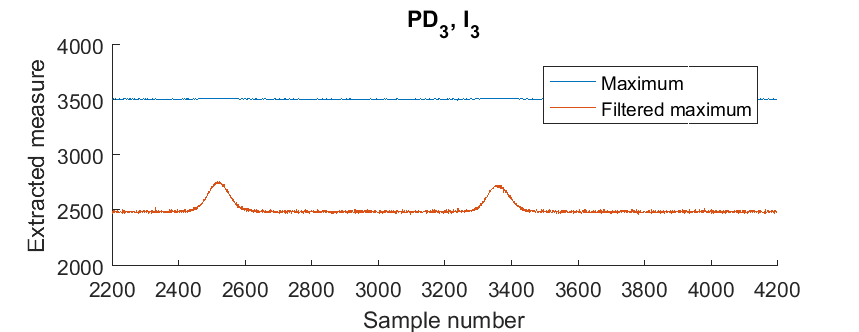
\includegraphics[width=60mm]{pics/SNR_simple_PD2.png}}
	\subfigure[]{\label{fig:simple_PD3}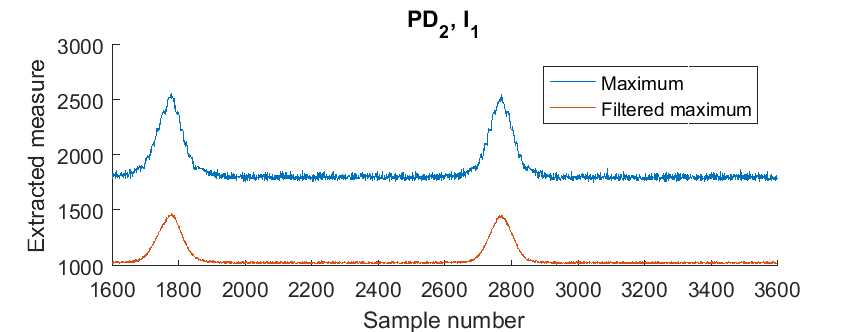
\includegraphics[width=60mm]{pics/SNR_simple_PD3.png}}
	\caption{Data extracted from consecutive flashes using the maximum and filtered maximum methods with $T_{on} = 250\mu s$.\label{fig:SimpleFeatures}}
\end{figure}

\begin{figure}
	\centering     %%% not \center
	\subfigure[]{\label{fig:complex_PD2}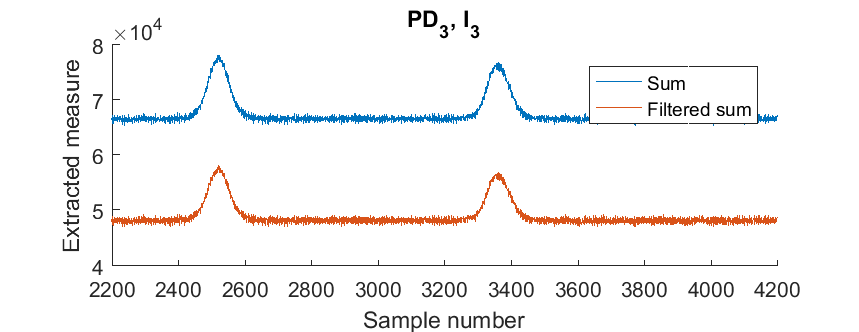
\includegraphics[width=60mm]{pics/SNR_complex_PD2.png}}
	\subfigure[]{\label{fig:complex_PD3}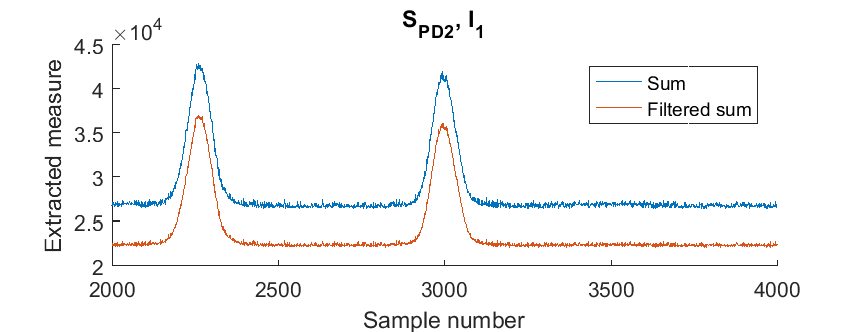
\includegraphics[width=60mm]{pics/SNR_complex_PD3.png}}
	\caption{Data extracted from consecutive flashes using the sum and filtered sum method with $T_{on} = 200\mu s$.\label{fig:complexFeatures}}
\end{figure}

\section{Flash period}
The final parameter to decide is the period of the signal, $T$. This value has no influence on the detectability of the signal. It has however a clear influence on how much light is used by the system, as decreasing $T$ directly increases the amount of flashes which occur. We can't choose a too low value for $T$ as then users will observe the flickering of the light. Another reason $T$ can't be chosen too low is that certain kind of noise still needs to be filtered out of the system. It is almost guaranteed that some 50Hz component will be seen in the signal, as long as it's connected to the net. 

For these reasons, $T$ was chosen to be 800$\mu s$ resulting in a flash frequency of 125Hz. This frequency is high enough to filter the expected 50Hz noise. Even though literature recommends at least 200Hz to prevent the visibility of flickering, none was observed by 10 different test subjects with this setting of $T$.

\section{Conclusion}
In this chapter, several methods of extracting useful data from a flashes where presented. 
The Flash analyser will run at a frequency of 125Hz, a $T_{on}$ of $200\mu s$ with maximum light intensity $I_1$ using the filtered sum method with $S_{PD_2}$ to extract information from the reflections. These settings provide the best found detectability with the given platform. The next step for the project is creating an algorithm to analyse set of consecutive flashes.